\chapter{Hintergrund} % Kapitel zum theoretischen Hintergrund
In diesem Abschnitt der Arbeit handelt, eine Basis des theoretischen Hintergrunds zu schaffen. Dieser Aspekt wird dadurch umgesetzt, indem zunächst auf die Kausalität dieses Projekt eingegangen wird - der Klimawandel (in Deutschland). Im nächsten Schritt muss der Begriff des Crowdsensings mit dem in der Literatur weitverbreiteten Begriff des Crowdsourcings abgegrenzt werden, um Unklarheiten im weiteren Verlauf dieser Arbeit zu vermeiden. Im Anschluss werden verwandte Arbeiten vorgestellt, welche sich mit dem Thema des Crowdsensings und der Umsetzung von Plattformen mit diesem Hintergrund beschäftigen.

\section{Der Klimawandel in Deutschland}
Der Klimawandel ist ein Thema, welches vor allem in den letzten Jahren verstärkt in den Fokus gerückt ist: Politische Entscheidungen\sidenote{vgl. Klimaschutzgesetz \cite{Klimaschutzgesetz}} berücksichtigen diesen, neue Produktvorstellungen werben mit verstärktem Recycling und der Produktion durch erneuerbare\sidenote{vgl. Release von neuen Apple Produkten und dem Ziel der Nachhaltigkeit unter \url{https://www.apple.com/de/environment/}} Energieträger. \\ Im Folgenden soll der Begriff des Klimawandels näher erläutert werden, um ein grundlegendes Verständnis für die Auswirkungen und die Notwendigkeit von Maßnahmen zu schaffen.

Dieser beschreibt das \textbf{Phänomen}, bei welchem sich treibhauswirksame Gase\sidenote{Beispiele für treibhauswirksame Gase: Methan und Distickstoffmonoxid (häufig in der Vieh- und Landwirtschaft), Kohlendioxid \cite{UmweltbundesamtKlimawandel}} in der Erdatmosphäre ansammeln und in der Tendenz zu einer Erwärmung der unteren Luftschichten führen \cite{UmweltbundesamtKlimawandel}. Dies hat zur Folge, dass sich das Klima seit dem vergangenen Jahrhundert erwärmt, sodass Auswirkungen in Form von Abnehmen von Gebirgsgletschern und Schneebedeckungen und das häufigere Auftreten von Extremereignissen wie Starkniederschläge und Hitzewellen beobachten werden können \cite{UmweltbundesamtKlimawandel}. Die Ursache für dieses Phänomen findet sich bei den Menschen, hauptsächlich durch die Verbrennung von fossilen Brennstoffen wie Kohle, Öl und Gas \cite{UnitedNationsClimateChange}. Bestätigt wird dieser Fakt dadurch, dass die Durchschnittstemperatur der Erdoberfläche 1,1°C heute wärmer ist als in den späten 1800er Jahren\sidenote{Zeit vor der industriellen Revolution} und damit den höchsten Stand in den letzten 100.000 Jahren \cite{UnitedNationsClimateChange} darstellt. Aufgrund dessen wird häufig vom sogenannten \textbf{anthropogenen}, also durch den Menschen verursachten Klimawandel gesprochen.

Auf den Menschen selbst wirkt sich der Klimawandel durch den Einfluss auf die menschliche Gesundheit, aber auch auf den Anbau von Nahrungsmitteln, die Behausung, die Sicherheit und das Arbeitsleben aus: \\ Häufig müssen Bewohner*innen von Küstenregionen aufgrund des steigenden Meeresspiegels umgesiedelt werden, da die Gefahr von Überschwemmungen steigt \cite{UnitedNationsClimateChange}. Auch die Versorgung mit Nahrungsmitteln ist durch den Klimawandel gefährdet, da die Ernteerträge durch die steigenden Temperaturen und die damit verbundene Trockenheit sinken \cite{UnitedNationsClimateChange}. Die Folgen des Klimawandels sind also nicht nur in der Zukunft zu erwarten, sondern bereits jetzt zu beobachten. \\ Verhindert werden soll das Voranschreiten durch die Reduzierung der Emissionen, der Adaption an die Auswirkungen des Klimas und dem Finanzieren von notwendigen Klimaschutzmaßnahmen. Die Reduzierung der Emissionen soll durch die Umstellung auf erneuerbare Energien, die Verbesserung der Energieeffizienz und die Reduzierung der Abholzung von Wäldern erreicht werden, während die Adaption durch die Anpassung an die Auswirkungen des Klimawandels, wie z.B. die Anpassung der Landwirtschaft an die veränderten Bedingungen, erarbeitet werden soll \cite{UnitedNationsClimateChange}. Die Finanzierung von Klimaschutzmaßnahmen soll durch die Unterstützung von Entwicklungsländern, die durch den Klimawandel besonders betroffen sind, aber nicht die nötigen finanziellen Mittel zum Reduzieren von CO2-Emissionen besitzen, erzielt werden \cite{UnitedNationsClimateChange}.


Doch auch in Deutschland kann die Änderung des Klimas beobachtet werden: Deutsche Wälder erleiden starke Schäden durch die Kombination von trockenen und heißen Tagen mit Stürmen, Starkregen und der Vermehrung des Borkenkäfers \cite{UmweltbundesamtRisikoanalyse2021}. Die Landwirtschaft ist abhängig von der Witterung einer Vegetationsperiode und einzelnen Wetterereignissen, da diese die Qualität und die Höhe des Ertrages bestimmen \cite{UmweltbundesamtRisikoanalyse2021}. Auch Tiere fühlen sich, wie Menschen, lediglich in einem bestimmten Temperaturbereich wohl, weswegen eine Überschreitung gesundheitliche Auswirkungen zur Folge hat \cite{UmweltbundesamtRisikoanalyse2021}. Die Auswirkungen fordern also die Notwendigkeit ein, Maßnahmen zu ergreifen, um den Klimawandel zu verlangsamen und die Auswirkungen zu minimieren.

\begin{marginfigure}[] % move figure up by 1 line 
    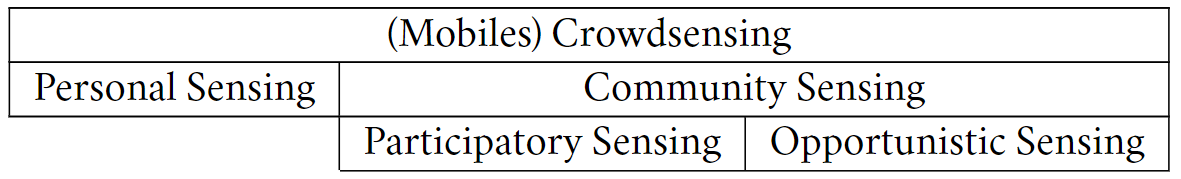
\includegraphics[width=1.1\marginparwidth]{figures/crowdsensing.png}
    \caption{\label{fig:crowdsensing}Unterteilung des Crowdsensings}
\end{marginfigure}

\section{Crowdsensing vs. Crowdsourcing}
\label{sec:crowdsensing}
In der Literatur wird der Begriff des \textbf{(mobilen) Crowdsensings} durch das Vorhandensein einer großen Anzahl an Teilnehmenden für eine großflächige Überwachung der Umwelt beschrieben, welche rohe Daten, mithilfe der in smarte Geräte eingebetteten Sensoren, messen \cite{Ray2022}. Um an den Begriff des Crowdsensings heranzutreten, wird aber zunächst zwischen zwei Arten des Messens unterschieden (vgl. Abbildung \ref{fig:crowdsensing}): dem sogenannten \enquote{personal sensing}, in dessen Anwendung Individuen persönliche Informationen aus eigenem Interesse oder Bedarf messen (z.B. Messungen zum Überwachen der eigenen Gesundheit, aber auch zum Nachverfolgen von persönlichen Rekorden oder dem ökologischen Fußabdruck) und dem \enquote{community sensing}, bei welchem großflächige Phänomene, welche durch einzelne Individuen nicht gemessen werden können, untersucht werden \cite{Ganti2011}. \\ Als Beispiele können hierfür sämtliche Anwendungsfälle genannt werden, in denen die Teilnahme von mehreren Individuen (unter Umständen zur selben Zeit) unabdingbar ist, wie beim Messen der Temperatur, der Luftfeuchtigkeit oder der Luftqualität an verschiedenen Orten. Die Rolle des \enquote{community sensing} kann hierbei weiterhin in zwei Kategorien unterteilt werden, dem \textbf{participatory sensing} \cite{Burke2006} und dem \textbf{opportunistic sensing} \cite{Lane2010}: \newline Während bei Ersterem eine aktive Teilnahme, verbunden mit eigenmotiviertem Aufwand (z.B. Aufnahme von Fotos, Eingabe und Übermittlung von Information), notwendig ist, wird bei Letzterem eher ein minimaler Aufwand durch eine selbstständige Messung der Sensoren (z.B. kontinuierliche Temperaturmessung der Sensoren in Abhängigkeit vom Standort, ohne Eingaben der Nutzer*innen) betrieben \cite{Ganti2011}. Aus diesem Grund bildet Crowdsensing in der Literatur keine eindeutige Art der Messung, sondern vielmehr eine Domäne der genannten Arten an Messungen durch eine Gruppe von Individuen \cite{Ganti2011}. \newline Das mobile Crowdsensing kann in drei Schritte gegliedert werden: der Datenerhebung, der -sammlung und dem -upload \cite{Ray2022}. Die Datenerhebung erfolgt sowohl durch die User, als auch durch \enquote{mobile sensing devices} (z.B. Thermometer, Smartphones etc.), welche auf einem Server gesammelt werden, um im Anschluss hochgeladen und einer Qualitätskontrolle unterzogen werden zu können \cite{Ray2022}. Die Vorteile des mobilen Crowdsensing erstrecken sich dabei von schneller Erhebung von vielfältigeren Daten mit erhöhter Qualität der Ergebnisse, bis hin zu akzeptableren Resultaten und dem Auslagern von Rechenleistung für die Erfassung der Daten von einer zentralen Plattform zu bspw. den mobilen Geräten \cite{Ray2022}. Auf der anderen Seite kann man jedoch beobachten, dass die erhobenen Daten geprägt von Redundanzen und Duplikaten sind, was zur Folge hat, dass eine anschließende Qualitätskontrolle und die Notwendigkeit von mehr Speicherplatz unabdingbar ist \cite{Ray2022}. Es lassen sich häufig Smartphones als Messgeräte des mobilen Crowdsensing in der Literatur finden, da diese mit einer vielzahl an Sensoren (Temperatur-, Gyroskop-, Umgebungslichtsensoren etc.) ausgestattet sind - das mobile Crowdsensing ist aber nicht auf diese limitiert und beinhaltet auch Geräte wie mobile Wetterstationen, Bewegungssensoren, Kameras o.Ä.


Das \textbf{mobile Crowdsourcing} ermöglicht das Lösen einer komplexen Herausforderung durch die Auf- und Verteilung von Aufgaben an eine Gruppe von freiwilligen Nutzer*innen, hier über das Internet \cite {Wang2019}. Die Komposition \textit{Crowdsourcing} besteht dabei aus den beiden einzelnen Wörtern \textit{crowd} für die (Menschen-)Menge und \textit{sourcing} für die Beschaffung (hier: von Informationen). Erstmalig wurde der Begriff 2006 vom Journalisten Jeff Howe in einem Artikel verwendet, welcher das Crowdsourcing als kostengünstigere Alternative des \textit{Outsourcing}\sidenote{zu deutsch: Auslagerung, \enquote{mittel- bis langfristige Übertragung von Aufgaben der Informationsverarbeitung eines Unternehmens an ein spezialisiertes Unternehmen} \cite{Heinrich2014}} beschreibt, um Akteure aus unterschiedlichen Wissensständen und Domänen in die Softwareentwicklung miteinzubinden \cite{Howe2006}. \\ Im weiteren Verlauf der Verwendung des Begriffs spielen die Charakteristiken ebenfalls eine Rolle: Die Lösung eines Problems wird insofern erreicht, dass die Aufgaben (und unter Umständen auch Unteraufgaben, abhängig von Problemstellung) an eine (Menschen-)Menge übertragen werden, welche interessiert an der Lösung des Problems ist \cite{Ray2022}. \\ Weiterhin wird die Verteilung der Menge und die Existenz von variierender Menschenlogik genutzt, um Probleme, an denen Computer scheitern, zu lösen \cite{Ray2022}. Der Unterschied zum Crowdsensing ist hierbei, dass die verrichtete Arbeit nicht auf die Interaktion mit Geräten und den entsprechenden Sensoren beschränkt ist, sondern dass Arbeit im Allgemeinen verrichtet wird (vergleiche Parallele zwischen Crowdsourcing und Outsourcing). Beim Einsatz vom mobilen Crowdsensing sind diverse Vorteile zu beobachten: Kosten für nicht benötigte Arbeitskräfte werden verringert (keine explizite Arbeitszeit vorhanden), die Datensammlung ist qualitativ hochwertiger und vielfältiger (durch Menge an Nutzer*innen) und Zeit wird durch die Verfügbarkeit von vielfältigen Parametern zum Testen gespart \cite{Ray2022}.


Aus den Definitionen der beiden Ausdrücke wird deutlich, dass diese viele Gemeinsamkeiten aufweisen, was der Grund dafür ist, dass in der Umgangssprache, aber auch in der Literatur, eine Verwechslung auftreten kann. Aufgrund dessen ist es erforderlich, die Abgrenzung der Begriffe voneinander hervorzuheben, welche sich in der Bearbeitung der Aufgaben und der Notwendigkeit von menschlicher Intelligenz befindet: Während das mobile Crowdsensing die Verantwortung auf das Erfassen von Rohdaten begrenzt, erstrecken sich diese beim Crowdsourcing über die Erfassung von Rohdaten bis zu anderen, von der Plattform zugewiesenen (allgemeinen) Aufgaben hinaus \cite{Ray2022}. Für eben diese wird dementsprechend auch eine bestimmte menschliche Intelligenz vorausgesetzt, die mit der Rechenleistung zusammenarbeiten soll, um eine Lösung zu finden \cite{Ray2022}.

\section{Verwandte Arbeiten}
\label{sec:related_work}
% Hier mit Verwandten Arbeiten vergleichen
Der Aspekt des Crowdsensing lässt sich sowohl in der Literatur, als auch in der Praxis durch bereits existierende Projekte und Anwendungen vorfinden. Um ein grundlegendes Verständnis über das Thema und zur Definition eines theoretischen Rahmens zu schaffen, werden diese verwandten Arbeiten herangezogen, welche in diesem Kapitel vorgestellt werden.

Bei der ersten Arbeit handelt es sich um \textit{Crowdsensing für Bodensee Online}, ein von der ISB AG, vom Fraunhofer-Institut für Optronik, Systemtechnik und Bildauswertung und der Ingenieurgesellschaft Prof. Kobus und Partner GmbH im Februar 2020 initiiertes Projekt zur Messung der Wassertemperatur des Bodensees durch Bootsbesitzer*innen mithilfe von mobilen Sensoren und Karten \cite {Ministerium2021}. Der Fokus des Projekts liegt darauf, die bereits vorhandenen Kenntnisse über die Verhältnisse am Bodensee durch einen citizen-science\sidenote{Bürger*innen werden in den Forschungsprozess miteinbezogen, wird hier als Synonym für Crowdsensing verwendet \cite{Heinisch2021}} Ansatz zu erweitern und auf die allgemeine Durchführbarkeit des Projekts zu messen \cite{Bodensee2021}. Dabei sollte zunächst in einer Pilotphase die Funktionsweise und die Montagemöglichkeit der Sensoren vor Ort erprobt werden, um im Anschluss mit ausgereiften Sensoren in die Feldphase zu starten, in welcher die Probanden mithilfe der Sensoren mit den Messungen des Bodensees beginnen konnten \cite{Bodensee2021}. Aufgrund der COVID-19 Pandemie und den damit vorherrschenden Einschränkungen verliefen beide Phasen teilweise zeitgleich, sodass eine kontinuierliche Weiterentwicklung der Sensoren und der Nutzeroberfläche basierend auf den Erfahrungen der Nutzer*innen möglich ist \cite{Bodensee2021}. Im Allgemeinen beschreiben die Durchführenden des Projekts die Ergebnisse als positiv. \newline In Bezug auf die technischen Aspekte soll der Betrieb, aber auch die Verfügbarkeit der Sensoren keinen Aufwand dargestellt haben. Auch die zuvor aufgestellten Anforderungen sind im breiten Maße erfüllt. Lediglich der Aufwand der Standortsuche der Sensoren und die damit verbundene Auswirkung auf die Batterielaufzeit haben eine wesentliche Limitierung dargestellt - eine erste Lösung ist aber dadurch umzusetzen, dass die Sensoren auch als stationäre Messpunkte (und einer erhöhten Anzahl) einzusetzen sind, um sowohl auf der einen Seite die Messdaten am Bodensee zu erhöhen, aber auf der anderen Seite die Abtastrate des Standortes zu minimieren, um die bereits erwähnten Limitierungen aufzuheben, sodass diese eine plausible Ergänzung zu den stationären Messstationen am Bodensee darstellen \cite{Bodensee2021}. \\ Der Crowdsensing-Ansatz des Projekts wird als geeignet für die Verbesserung und Verfeinerung einer bestehenden (Daten-)Struktur angesehen, da unter der Voraussetzung einer ausreichenden Qualitätssicherung und Datenmenge eine hohe Datenqualität und -dichte auf engem Raum erzielt werden kann \cite{Bodensee2021}. Prinzipiell ließe sich das Projekt laut Angaben der Durchführenden auf weitere (Naturschutz-)Regionen unter Zuhilfenahme weiterer Parameter (z.B. Lufttemperatur, -feuchtigkeit, -qualität) übertragen \cite{Bodensee2021}. Die zugrundeliegenden Charakteristiken lassen darauf schließen, dass es sich bei \textit{Crowdsensing für Bodensee Online} um \textbf{opportunistic sensing} handelt, da die Sensoren lediglich an die Boote angebracht werden müssen und keine aktive Teilnahme der Bootsbesitzer*innen notwendig ist.

Aber auch in anderen Domänen ist das Crowdsensing schon zum Einsatz gekommen: Das Projekt \textit{Track Your Tinnitus}\sidenote{https://www.trackyourtinnitus.org/de/} wurde von der Tinnitus Research Initiative (TRI) und dem Institut für Datenbanken und Informationssysteme (DBIS) der Universität Ulm für medizinische Einsatzzwecke 2013 ins Leben gerufen \cite{Pryss2017}. Etwa 10-15\% der Weltbevölkerung leidet unter Tinnitus, einer Krankheit, die durch ein ständiges Ohrgeräusch gekennzeichnet ist und welche bis heute schwer behandelbar ist, da verfügbare Behandlungen nur bei einem Teil der Betroffenen anschlagen \cite{langguth2011review}. Da klinische Tests und Versuche bisher den Standard repräsentiert haben, und die damit verbundene Informationsgewinnung begrenzt ist, wurde das Projekt ins Leben gerufen, um eine komplementäre Vorgehensweise vorzuschlagen, die durch den Einsatz von Crowdsensing-Services die Datenerhebung vereinfacht, aber auch vervielfacht \cite{pryss2015mobile}. Die Nutzer*innen sollen dabei eine Smartphone-App installieren und nach jedem Wahrnehmen des Tinnitus Fragen zur Intensität und Belastung und daraus resultierend, die Auswirkungen auf die persönliche Stimmungslage beantworten, damit individuelle Schwankungen der Tinnituswahrnehmung erfasst werden können \cite{pryss2015mobile}. \\ Einerseits soll es auf diese Weise ermöglicht werden, die behandelnden ärztlichen Fachpersonen mit den notwendigen Daten zu versorgen, um die Behandlung zu verbessern, aber auch das allgemeine Forschungsprojekt zu unterstützen und ein Verständnis für Ursachen und Wirkungen für den Tinnitus zu schaffen \cite{pryss2015mobile}. Die Voraussetzung der Eingabe der persönlichen Tinnituswahrnehmung charakterisiert das Projekt \textit{Track Your Tinnitus} als \textbf{participatory sensing}, da die Nutzer*innen aktiv an der Datenerhebung beteiligt sind.

Eine weitere verwandte Arbeit ist die Applikation \textit{Budburst}\sidenote{https://budburst.org}, welche Nutzer*innen dazu animiert, mithilfe des eigenen Mobiltelefons Pflanzenarten zu identifizieren und in einer Gemeinschaft lokale Pflanzen(-arten) kontinuierlich zu erfassen. Die Nutzer*innen werden durch die kontinuierliche Erfassung der Pflanzen dazu animiert, den Zustand des lokalen Ökosystems zu überwachen um eventuelle Rückschlüsse auf den Klimawandel ziehen zu können. Durch das Fotografieren von Pflanzen innerhalb der App soll ein Diskurs über die Gesundheit des Ökosystems angeregt werden, welcher durch die Nutzer*innen und die daraus geformte Gemeinschaft geführt wird. Die App \textit{Budburst} ist ein Beispiel für \textbf{participatory sensing}, da die Nutzer*innen ebenfalls aktiv an der Datenerhebung beteiligt sind.

Ausgehend von den genannten Arbeiten und Projekten ist es möglich, weitere verwandte Quellen zu finden, welche sich mit dem Thema des Crowdsensings beschäftigen. Die genannten Arbeiten haben dabei gezeigt, dass das Crowdsensing in unterschiedlichen Domänen zum Einsatz kommen kann, um Problemstellungen zu lösen, welche durch traditionelle Methoden nicht oder nur schwer zu lösen sind. Alle vorgestellten Arbeiten stellen Softwarelösungen dar, die durch Eingaben von Nutzer*innen Daten erheben oder diese evaluieren und in der Regel zu einer Verbesserung der Qualität beitragen sollen. Dabei werden durch die verwandten Arbeiten unterschiedliche Einsatzzwecke abgedeckt. Diese Arbeit soll keine der genannten Arbeiten oder ihren Einsatzzweck ersetzen, sondern sich vielmehr in diese Liste der Crowdsensing-Lösungen einreihen und den Ansatz mithilfe der Kuratierung der Umweltdaten in Bamberg näherbringen, da ein solches Projekt bisher nicht existiert.